\pdfinfoomitdate=1
\pdftrailerid{}
\documentclass[tikz,border=4pt]{standalone}
\usepackage{newtxtext}
\usetikzlibrary{arrows.meta,positioning}
\definecolor{blue}{HTML}{0072B2}
\definecolor{orange}{HTML}{E69F00}
\definecolor{green}{HTML}{009E73}
\definecolor{graybox}{HTML}{F0F0F0}
\tikzset{
  box/.style={draw=black,rounded corners=2pt,very thick,minimum width=60mm,
    minimum height=43mm,align=left,text width=52mm,font=\sffamily\small,
    inner sep=4mm},
  arrow/.style={-{Latex[length=3mm]},very thick}
}
\begin{document}
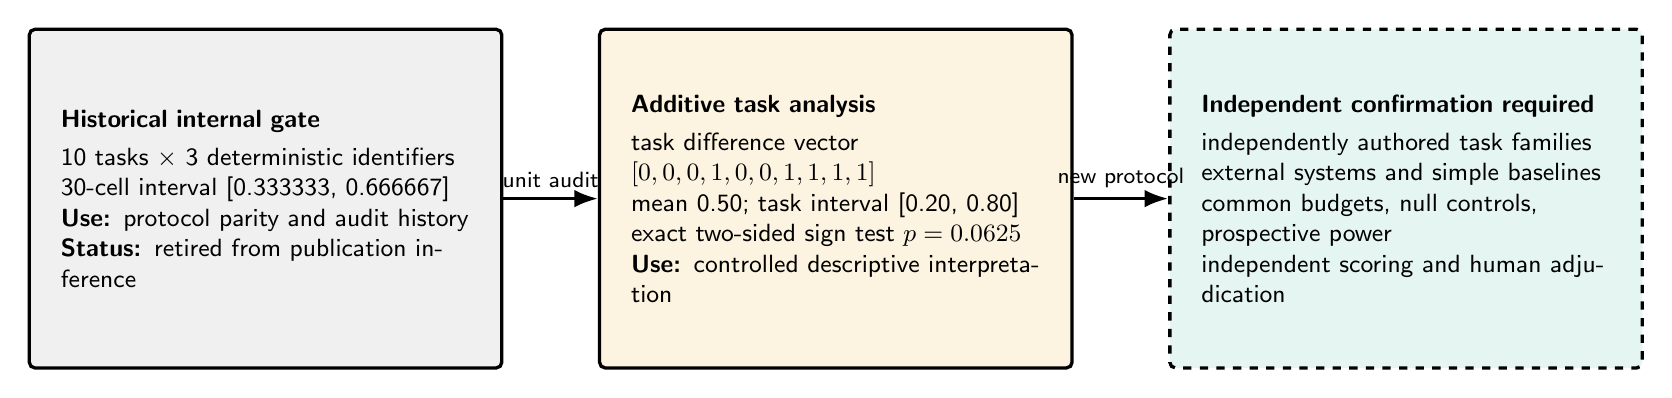
\begin{tikzpicture}[node distance=12mm]
  \node[box,fill=graybox] (history) {\textbf{Historical internal gate}\\[1mm]
    10 tasks $\times$ 3 deterministic identifiers\\
    30-cell interval [0.333333, 0.666667]\\
    \textbf{Use:} protocol parity and audit history\\
    \textbf{Status:} retired from publication inference};
  \node[box,fill=orange!12,right=of history] (correction) {\textbf{Additive task analysis}\\[1mm]
    task difference vector $[0,0,0,1,0,0,1,1,1,1]$\\
    mean 0.50; task interval [0.20, 0.80]\\
    exact two-sided sign test $p=0.0625$\\
    \textbf{Use:} controlled descriptive interpretation};
  \node[box,fill=green!10,right=of correction,dashed] (future) {\textbf{Independent confirmation required}\\[1mm]
    independently authored task families\\
    external systems and simple baselines\\
    common budgets, null controls, prospective power\\
    independent scoring and human adjudication};
  \draw[arrow] (history) -- node[above,font=\sffamily\footnotesize] {unit audit} (correction);
  \draw[arrow] (correction) -- node[above,font=\sffamily\footnotesize] {new protocol} (future);
\end{tikzpicture}
\end{document}
